\documentclass[10pt,twoside,letterpaper]{book}
\usepackage[T1]{fontenc}
\usepackage{bookman}
\usepackage{color}
\usepackage{amsmath}
\usepackage{amsfonts}
\usepackage[active]{srcltx}
\usepackage{graphicx}
\usepackage{float}
\usepackage{multirow}
\usepackage{verbatim}
\usepackage[small,bf]{caption}
\usepackage{wrapfig}

%\usepackage[colorlinks]{hyperref}
\usepackage[colorinlistoftodos, textwidth=3cm, textsize=tiny, shadow]{todonotes}
\usepackage[pdftex,
  pdfauthor={AICML},
  pdftitle={BioBank Client User Guide},
  colorlinks,
  linkcolor=blue,
  bookmarks=true,
  bookmarksopen=true,
  pdfstartview=FitH]
	   {hyperref}

\DeclareMathAlphabet{\mathpzc}{OT1}{pzc}{m}{it}

% no indentation at beginning of paragraph, and 1 line separating paragraphs
\setlength{\parindent}{0pt}
\setlength{\parskip}{1ex}

\oddsidemargin  0.0in
\evensidemargin 0.0in
\textwidth      6.0in
\headheight     0.0in
\topmargin      0.0in
\textheight     9.0in
\setlength{\marginparwidth}{0.8in}
\let\oldmarginpar\marginpar

\setcounter{secnumdepth}{3}

\begin{document}
\frontmatter

\title{BioBank Client User Guide}
\author{\Large{Prepared for the Canadian BioSample Repository}\\
by the Alberta Innovates Centre for Machine Learning}
\maketitle
\clearpage
\tableofcontents
\clearpage
\listoffigures
\clearpage
\listoftodos
\clearpage

\mainmatter
\chapter{Overview}
The BioBank2 Java Client is designed to be a client application that connects
to a server which provides services for storing inventory information for
biological samples. More than one client can connect to the server at the same
time. The client is a software application that runs on Microsoft Windows and
Linux\footnote{The scanner cannot be used when using the application on Linux.}. The client
software is a Java application and requires that a Java JRE or JDK be installed
on the computer. The installation program for the client installs a Java JRE if
it is not already present on the computer.

When running on Microsoft Windows, the client can connect to scanners use either
TWAIN\footnote{\url{http://en.wikipedia.org/wiki/TWAIN}} or
WIA\footnote{\url{http://en.wikipedia.org/wiki/Windows_Image_Acquisition}}
drivers. Most scanners available on the market provide these
drivers. Therefore, most scanners work with the client software.

Figure \ref{fig:main_window} shows the application's main window and highlights
different some of its components.
    \begin{figure}[H]
      \centering
      \scalebox{0.4}
      { \includegraphics*{screenshots/overview/main_window} }
      \caption{The Java Client's main window.}
      \label{fig:main_window}
    \end{figure}
\begin{description}
  \item[Main Menu] The main menu allows the user access to the different
    functions provided by the software (see section \ref{sec:main_menu} for a
    description of the menu items). The application also has an icon based
    toolbar to access commonly used functions.
  \item[Toolbar Icons] The icon buttons in the toolbar allow quick access to
    often used menu items. Using the mouse, the user can hover over the icon
    button and after 2 seconds a tooltip is displayed describing what the
    button is for and if applicable the keyboard shortcut. Note that there is
    an icon toolbar under the Main Menu and another grouped with the tree view.
  \item[Tree View] The tree view shown here is for the \emph{Administration
    View}. The application uses tree views in the \emph{Administration View}
    and \emph{Processing View} (see section \ref{sec:application_views}). Tree
    view shows nodes in a hierarchical structure. If a node has children a
    \emph{plus} symbol is displayed next to the node. When the symbol is
    pressed the node will expand to show its' child nodes.  Sometimes,
    operations can be performed on certain nodes in the tree by right clicking
    with the mouse on the node.
  \item[Status Bar] The status bar is used to display the current state of the
    application. It is usually updated after the user has completed a task.
\end{description}

\section{Main Menu}
\label{sec:main_menu}

\subsection{Server}
The child menu items of the \emph{Server} main menu item allow the user to
login or logout from a server and to quit the application.
    \begin{figure}[H]
      \centering
      \scalebox{0.5}
      { \includegraphics*{screenshots/overview/main_menu_server} }
      \caption{Server menu.}
      \label{fig:main_menu_server}
    \end{figure}
\begin{description}
  \item[Login] This menu item allows the user to login to a BioBank2 server. On
    startup and when logged out this menu item is enabled. When logged into a
    server this menu item is disabled. Also, the \mbox{\fbox{Ctrl} + \fbox{L}}
    keyboard short cut can be used to perform this function.
\end{description}

\subsection{Administration}
\subsection{Processing}
\subsection{View}
\subsection{Print}
\subsection{Scanner}
\subsection{Search}
\subsection{Configuration}
\subsection{Help}

\section{Views}
\label{sec:application_views}

\chapter{Configuration}
The configuration settings for the Java Client can be found by selecting
\texttt{Configuration -> Preferences} from the main menu.
    \begin{figure}[H]
      \centering
      \scalebox{0.5}
      { \includegraphics*{screenshots/configuration/preferences_dialog} }
      \caption{Configuration preferences dialog box.}
      \label{fig:preferences_dialog}
    \end{figure}
A configuration page can be selected by clicking on a node on the
tree on the left hand side of the dialog box. The \texttt{filter text} box, see
arrow labelled \emph{1} in figure \ref{fig:preferences_dialog}, can
be used to quickly find a configuration page by typing the name of the page in
whole or in part.

The following sections discuss the configuration pages in detail.

\section{Automatic Updates}
The Java Client has the capability of detecting when a new version of the
software has been made available by the software design team. The settings on
this page allow the user to specify when updates will be searched for, when to
download them, and how to notify the user when they are found.

\section{General}
The settings on this page are general to the application.
    \begin{figure}[H]
      \centering
      \scalebox{0.5}
      { \includegraphics*{screenshots/configuration/prefs_general} }
      \caption{General preferences.}
      \label{fig:prefs_general}
    \end{figure}
\begin{description}
  \item[Show software version in main window title] the Java Client's software
    version can be displayed in the window's title bar by checking this
    box.\textit{Note that this option is only required by technicians when they
      are testing new versions of the software}.
  \item[Show heap status] the \emph{heap status} can be displayed in the main
    window by checking this box. The heap status gives an indication of the
    memory used by the application. \textit{This option is in place for the
      software designers and is not required for normal use}.
\end{description}

\section{Issue Tracker}
The application has the capability of sending \emph{Problem Report} emails to
the software design team\footnote{\texttt{Help -> Send Error Email} from the
  main menu}. The error emails have application state information attached to
aid team in resolving potential problems. The settings on this page are the
settings used to send the emails to the team.
    \begin{figure}[H]
      \centering
      \scalebox{0.5}
      { \includegraphics*{screenshots/configuration/prefs_issue_tracker} }
      \caption{Issue tracker preferences.}
      \label{fig:prefs_issue_tracker}
    \end{figure}
\begin{description}
  \item[Tracker email] The email address to send problem reports to.
  \item[SMTP server] The SMTP mail server to use when sending emails.
  \item[SMTP server port] The SMTP server port.
  \item[SMTP server username] The user name to use with the SMTP server.
  \item[SMTP server password] The password to use with the SMTP server.
\end{description}
\textit{Users should not modify these settings unless requested to by the software
  design team}.

\section{Link \ Assign}
These settings are used when scanning and decoding pallets and linking them to
patients or container locations.
\marginpar{\color{red}{There should  be an appendix with instructions on how to create
  these barcodes.}}
    \begin{figure}[H]
      \centering
      \scalebox{0.5}
      { \includegraphics*{screenshots/configuration/prefs_link_assign} }
      \caption{Scan link / Assign preferences.}
      \label{fig:prefs_link_assign}
    \end{figure}
\begin{description}
  \item[Confirm Barcode and Cancel Barcode] To speed up
    processing of samples, a handheld barcode scanner can be used to quickly
    enter information into the application. Barcodes with the corresponding
    words can be printed and then scanned when required by the application (See
    sections \ref{sec:scan_link}, \ref{sec:scan_assign} and
    \ref{sec:cabinet_scan_link_assign}). The \textbf{Confirm Barcode} and
    \textbf{Cancel Barcode} settings contain the text encoded into these
    barcodes when they were created.
  \item [Save activity logs into a file and Path for activity logs files] When
    processing patients, the actions taken by the user can be logged and saved
    to files on disc. This section allows the user to activate saving this
    logging to disc and specify the path on disc where the files are will be
    saved.
  \item[\textbf{Ask to print activity log}] When a scan link or scan assign
    session is over the user can be prompted to print the activity logs. This
    setting enables or disables the prompting.
\end{description}

\section{Scanning and Decoding}
The settings on this page allow the user to specify the scanning and
decoding parameters used when decoding pallet images.
    \begin{figure}[H]
      \centering
      \scalebox{0.5}
      { \includegraphics*{screenshots/configuration/prefs_scanning_and_decoding} }
      \caption{Scanning and Decoding preferences.}
      \label{fig:prefs_scanning_and_decoding}
    \end{figure}
\begin{description}
  \item[Select Scanner] This button is used to select the scanner that will be
    used to scan 96 well pallets. The dialog box shown in figure
    \ref{fig:prefs_select_source} is shown when the button is pressed.
    \begin{figure}[H]
      \centering
      \scalebox{0.5}
      { \includegraphics*{screenshots/configuration/prefs_select_source} }
      \caption{Selecting a scanning source.}
      \label{fig:prefs_select_source}
    \end{figure}
  \item[Driver Type] The type of driver that was selected when the \fbox{Select
    Scanner} button was pressed. Normally, the application will attempt to
    determine the driver type as soon as the user makes the selection, but
    sometimes the application does not select the correct type. Use the check
    boxes here to override what the application selected.
  \item[DPI] The \emph{Dots per Inch} used by the scanner for scanning
    images. For best results use 600 DPI.
  \item[Brightness] The brightness setting to be used when scanning
    images. This parameter does not work on Hewlett-Packard scanners when using
    the WIA based driver.
  \item[Contrast] The contrast setting to be used when scanning
    images. This parameter does not work on Hewlett-Packard scanners when using
    the WIA based driver.
\end{description}

\subsection{Decoding Parameters}
On the preferences dialog window, if there is a "plus" symbol next to the
\emph{Scanning and Decoding} node, press it to expand the sub tree.

These settings control how the software decodes the sample tubes imprinted with
DataMatrix 2D barcodes.
    \begin{figure}[H]
      \centering
      \scalebox{0.5}
      { \includegraphics*{screenshots/configuration/prefs_decoding_parms} }
      \caption{Decoding preferences.}
      \label{fig:prefs_decoding_parms}
    \end{figure}
\begin{description}
  \item[Decode Library Debug Level] The decoding software library can output
    debugging information to a log file. When this value is zero there is no
    debugging information stored in the log file. Possible values are 0 through
    9. The higher the value the more detailed the debugging information.
  \item[Decode Edge Threshold] Set the minimum edge threshold as a percentage
    of maximum. For example, an edge between a pure white and pure black pixel
    would have an intensity of 100.  Edges with intensities below the indicated
    threshold will be ignored by the decoding process. Lowering the threshold
    will increase the amount of work to be done, but may be necessary for low
    contrast or blurry images. The default and recommended value is \emph{5}.
  \item[Decode Square Deviation] Maximum deviation (in degrees) from squareness
    between adjacent barcode sides. The default and recommended value is
    \emph{N=15} and is meant for scanned images. Barcode regions found with
    corners \emph{<(90-N)} or \emph{>(90+N)} will be ignored by the decoder.
  \item[Decode Corrections] The number of corrections to make while
    decoding. The default and recommended value is 10.
  \item[Decode Scan Gap] The scan grid gap size in inches. The default and
    recommended value is \emph{0.085}.
  \item[Decode Cell Distance] The distance in inches between tubes.The default
    and recommended value is \emph{0.345} for NUNC pallets.
\end{description}

\subsection{Decoding Profiles}
On the preferences dialog window, if there is a "plus" symbol next to the
\emph{Scanning and Decoding} node, press it to expand the sub tree.

This page allows the user to define \emph{Decoding Profiles}. These profiles
allow the user define a sub set of tubes to decoded when an image of a pallet
is scanned. Scanning profiles can be used during scan link and scan assign (see
sections \ref{sec:scan_link} and \ref{sec:scan_assign}).
    \begin{figure}[H]
      \centering
      \scalebox{0.45}
      { \includegraphics*{screenshots/configuration/prefs_decoding_profiles} }
      \caption{Decoding profiles preferences.}
      \label{fig:prefs_decoding_profiles}
    \end{figure}
For example: the user may wish to only decode every other row on a pallet. Once
the profile is created it can be used at scan link and scan assign time and
only the cells activated in the profile will be decoded. If 2D barcodes are
found in the cells not active in the profile, the user will be given a warning
message.

To create a new profile follow these instructions:
\begin{enumerate}
  \item Press the \fbox{Add...} button. A dialog box pops up requesting a name
    for the new profile. Enter an appropriate name and press the \fbox{OK}
    button.
  \item Now select each cell that should be part of the profile (see cells with
    a checkmark in Figure \ref{fig:prefs_decoding_profiles}). When done
    selecting cells press the \fbox{Apply} button.
\end{enumerate}

\subsection{Plate Positions}
On the preferences dialog window, if there is a "plus" symbol next to the
\emph{Scanning and Decoding} node, press it to expand the sub tree.
    \begin{figure}[H]
      \centering
      \scalebox{0.5}
      { \includegraphics*{screenshots/configuration/plate1_definition} }
      \caption{Configuring a plate position.}
      \label{fig:plate1_definition}
    \end{figure}

To define a pallet scanning region do the following:
\begin{enumerate}
  \item Place a pallet that contains tubes on the flatbed scanner. Ensure the
    top edge of the pallet is touching the top of the scanning region, and the right
    edge of the pallet is touching the right margin. Ensure the 12 columns
    are vertical and the 8 rows are horizontal.
  \item Select the plate region you are going to define.  If it is the first
    select \emph{Plate 1 Position}.
  \item Click on the "Enable" box.
  \item Press the \fbox{Scan} button. Now wait for the scanner to scan the entire
    flatbed.
    \begin{figure}[H]
      \centering
      \scalebox{0.5}
      { \includegraphics*{screenshots/configuration/sample_flatbed_scan} }
      \caption{Sample flatbed scan.}
      \label{fig:sample_flatbed_scan}
    \end{figure}
  \item Once the scan is done, you will see something similar to Figure
    \ref{fig:sample_flatbed_scan}. The image shown on the right hand side is
    the image taken by the scanner and superimposed is a grid with 8 rows and
    12 columns. The cell coloured in cyan should correspond to tube in row A and
    column 1.
  \item Under orientation select "Landscape".
  \item You can adjust the size of the grid using the mouse. If you move the
    mouse to one of the corners or one of the edges you can resize the grid by
    holding down the left button on the mouse. The whole grid can be moved by
    pressing the left mouse button while hovering inside the grid.
  \item Once the grid cells are aligned with each tube press the \fbox{OK} button
    (see Figure \ref{fig:plate1_grid_ready}). The wheel on the mouse can be
    used to make the cells smaller or bigger (this is referred to as the
    \emph{Cell Gap}).
    \begin{figure}[H]
      \centering
      \scalebox{0.5}
      { \includegraphics*{screenshots/configuration/plate1_grid_ready} }
      \caption{Grid aligned with tubes.}
      \label{fig:plate1_grid_ready}
    \end{figure}
  \item Repeat from step 2 to define any more pallet scanning regions.
  \item Usually only one pallet scanning region is required for normal
    operation of the software.
\end{enumerate}
Figure \ref{fig:plate2_grid_ready} shows an example of how \emph{Plate 2} can
be defined. Here Plate 2 is touching the top and the left margin of
the of the flatbed region. The plate on the left of the image is where Plate 1
is defined.
    \begin{figure}[H]
      \centering
      \scalebox{0.5}
      { \includegraphics*{screenshots/configuration/plate2_grid_ready} }
      \caption{Plate 2 grid aligned with tubes.}
      \label{fig:plate2_grid_ready}
    \end{figure}
Note that cell A1 should be at the \emph{Top Left} when configuring a plate in
\textbf{Landscape} orientation and \emph{Top Right} when in \textbf{Portrait}
orientation when looking down at the scanner's flatbed.

To test if your configuration will yield valid decodes use the
\texttt{Scanner -> Decode Plate} from the main menu.
\subsection{Plate Barcodes}
To speed up processing of samples, a handheld barcode scanner can be used to
quickly enter information into the application. Barcodes with the corresponding
words can be printed and then scanned when required by the application (See
sections \ref{sec:scan_link} and \ref{sec:scan_assign}). The \textbf{Plate
  \emph{x} barcode} settings contain the text encoded into these barcodes when
they were created.
    \begin{figure}[H]
      \centering
      \scalebox{0.45}
      { \includegraphics*{screenshots/configuration/prefs_plate_barcodes} }
      \caption{Plate barcode preferences.}
      \label{fig:prefs_plate_barcodes}
    \end{figure}

\section{Servers}
This page contains a list of BioBank2 servers that the Java Client connects to
on a regular basis. This list is used in the login dialog box to aid the user
to quickly select a server. New servers can be added to this list by pressing
the \fbox{New} button. Only the domain name or IP address for the server is
required.
    \begin{figure}[H]
      \centering
      \scalebox{0.45}
      { \includegraphics*{screenshots/configuration/prefs_servers} }
      \caption{Server preferences.}
      \label{fig:prefs_servers}
    \end{figure}

Previously entered servers can also be edited with the \fbox{Edit} button if a
spelling mistake was made.

The order in the list can be rearranged with the \fbox{Up} and \fbox{Down}
buttons to put more frequently accessed servers at the beginning of the list.



\chapter{Patient Processing}

\section{Shipment}

\section{Patient Visit}

\section{Scan Link}
\label{sec:scan_link}

\section{Scan Assign}
\label{sec:scan_assign}

\section{Cabinet Link and Assign}
\label{sec:cabinet_scan_link_assign}

\section{Patient Merging}

\chapter{Sample Order Processing}

\chapter{Dispatch}
The \emph{Dispatch} feature is used to record the shipping of a set of patient
sample aliquots between two repository sites where all patients and aliquots
belong to a single study.  Aliquots from multiple patients may be included in a
dispatch.

To use the dispatch feature in BioBank2 the two sites and the study involved
must first be configured (see section \ref{sec:config_send} for instructions).

Prior to sending a dispatch, the administrator of the sending site must create
a \emph{dispatch entry} that records the aliquots that are part of the
shipment. After the entry is created and the dispatch is ready to be sent, the
administrator must mark the entry as Sent. At this point BioBank2 displays the
dispatch entry as In Transit (see section \ref{sec:dispatch_send}).

Sites that wish to send dispatches can only send aliquots that have been scan
assigned to container positions. Aliquots without a position are not allowed in
a dispatch.

When receiving a dispatch, a technician with the appropriate role must Receive
and Process the dispatch entry in BioBank2. Only entries marked as In Transit
can be received and processed. A technician has the option of only marking an
entry as received and then process it at a later time. Processing of a dispatch
entry involves confirming that the aliquots recorded as sent are actually
received. See section \ref{sec:dispatch_receive} for instructions.  The
following errors can happen when sending a dispatch:
\begin{itemize}
  \item The shipment never arrives at the destination site.
  \item One or more aliquots marked as sent are not actually received at the
    receiving site,
  \item One or more aliquots never marked as sent are received at the receiving
    site.
\end{itemize}
Please see sections \ref{sec:dispatch_not_arrive},
\ref{sec:dispatch_missing_aliquots} and \ref{sec:dispatch_extra_aliquots} for
instructions on how to deal with these cases.  If a repository site no longer
sends dispatches, the instructions to remove the dispatche information is given
in section \ref{sec:config_send_remove}.
\section{Configure a Site for Sending Dispatches}
\label{sec:config_send}
\begin{enumerate}
  \item Log into the BioBank2 Java Client as a user in the Website
    Administrator group.
  \item From the Administration view, edit the site that is to send dispatches.
  \item \label{add_dispatch} Click on Add Dispatch Relation (see Figure
    \ref{fig:dispatch_add_configuration}).
    \begin{figure}[H]
      \centering
      \scalebox{0.5}
      { \includegraphics*{screenshots/dispatch_add_configuration} }
      \caption{Configuring a site for sending dispatches.}
      \label{fig:dispatch_add_configuration}
    \end{figure}
  \item From the dialog box the pops up, select the study associated with the
    site and the destination site for the shipments (see Figure
    \ref{fig:dispatch_add_config_dest_site}) and press the \emph{OK}
    button. Use the buttons with arrows to move a site from the \emph{Available
      Sites} to the \emph{Selected Destination Sites} boxes.
    \begin{figure}[H]
      \centering
      \scalebox{0.5}
      { \includegraphics*{screenshots/dispatch_add_config_dest_site} }
      \caption{Configuring the destination site for dispatches.}
      \label{fig:dispatch_add_config_dest_site}
    \end{figure}
  \item If there are more studies that dispatch from this site go to step \ref{add_dispatch}.
\end{enumerate}
\section{Remove Dispatch Configuration for a Site}
\label{sec:config_send_remove}
\begin{enumerate}
  \item Log into the BioBank2 Java Client as a user in the Website
    Administrator group.
  \item From the Administration tree view, right click on the site that will no longer send
    dispatches and select \emph{Edit Site}.
  \item In the entry form that opens up, right click on the study / site you
    wish to remove the configuration for and select \emph{Delete}.
    \begin{figure}[H]
      \centering
      \scalebox{0.5}
      { \includegraphics*{screenshots/dispatch_del_config} }
      \caption{Removing dispatch configuration for a site.}
      \label{fig:dispatch_del_config}
    \end{figure}
\end{enumerate}
\section{Sending a Dispatch}
\label{sec:dispatch_send}
\begin{enumerate}
  \item Log into the BioBank2 Java Client as a user in the Website
    Administrator group ({\color{red} which user groups should be allowed to
      create dispatches?}).
  \item In the \emph{Working Site} pull down, select the site that is to send the
    dispatch.
  \item Using the main menu or the toolbar icon select \emph{Dispatch} view.
  \item Select \emph{Add Dispatch} from the \emph{Dispatch Shipments} sub menu
    or from the toolbar icon.
    \begin{figure}[H]
      \centering
      \scalebox{0.5}
      { \includegraphics*{screenshots/dispatch_add} }
      \caption{Creating a new dispatch.}
      \label{fig:dispatch_add}
    \end{figure}
  \item Select the study and receiver site the dispatch aliquots are for. If
    there is a single study and / or a single receiver site they will be
    already selected.
    \begin{figure}[H]
      \centering
      \scalebox{0.5}
      { \includegraphics*{screenshots/dispatch_add_entry} }
      \caption{Selecting study and site when creating a dispatch.}
      \label{fig:dispatch_add_entry}
    \end{figure}
  \item Press the \emph{open scan dialog} button to scan assign aliquots into
    the dispatch and the following dialog box is displayed.
    \begin{figure}[H]
      \centering
      \scalebox{0.35}
      { \includegraphics*{screenshots/dispatch_add_entry_scan} }
      \caption{Scanning aliquots into a dispatch.}
      \label{fig:dispatch_add_entry_scan}
    \end{figure}
  \item Enter the pallet's product barcode or click the \emph{new
    pallet}\footnote{The new pallet check box is used when aliquots are moved
    from their original pallet to a new pallet to be used for the actual shipping.} check
    box, then the plate number for where the pallet has been placed on the
    flatbed scanner and then press the Launch Scan button.
\end{enumerate}
\section{Receiving a Dispatch}
\label{sec:dispatch_receive}
\section{Dispatch Never Arrives at Destination Site}
\label{sec:dispatch_not_arrive}
\section{Dispatches with Missing Aliquots}
\label{sec:dispatch_missing_aliquots}
\section{Dispatch with Extra Aliquots}
\label{sec:dispatch_extra_aliquots}

\chapter{Administration}
\label{chap:administration}

\section{Repository Sites}
\section{Clinics}
\section{Studies}
\section{Container Types}
\section{Containers}
\section{Moving Samples Between Containers}
\section{Sample Types}
\section{Source Vessels}
\section{Shipping Methods}
\section{Activity Status}
\section{User Management}

You can open the user/group administration dialog by selecting
\texttt{Administration} $\to$ \texttt{User Management}.
This menu is available only if you are a super administrator or administrator 
of your working center. 

You will see the dialog shown in \ref{fig:user_management}. It allows you to 
add/delete/edit users and groups. If you are not super administrator, you will 
only see users and groups of your current working center.
\begin{figure}[H]
  \centering
  \scalebox{0.5}
	   { \includegraphics*{screenshots/administration/user_management} }
	   \caption{User management dialog.}
	   \label{fig:user_management}
\end{figure}

\subsection{Adding Users}
To add a new user, open the User Management dialog and click on the \fbox{+} button
of the users section. You will see the following dialog window pop up. Enter the 
user's details and press the \fbox{OK} button.

A user should be assigned to at least one group. The centres assigned to these groups
become the 'working centres' of the user.

The password assigned to the new user is temporary. When the user logs in for
the first time, he/she will be asked to enter the temporary password and
select a new password.
\begin{figure}[H]
  \centering
  \scalebox{0.5}
	   { \includegraphics*{screenshots/administration/add_user} }
	   \caption{Adding a user.}
	   \label{fig:add_user}
\end{figure}


\subsection{Modifying Users}
To modify a user, open the User Management dialog, right click on the user and select 
edit or delete on the pop-up. If edit is selected, then the same dialog as in \ref{fig:add_user} is displayed.
\begin{figure}[H]
  \centering
  \scalebox{0.5}
	   { \includegraphics*{screenshots/administration/edit_delete_user} }
	   \caption{Pop-up to edit or delete users.}
	   \label{fig:edit_delete_users}
\end{figure}


\subsection{Adding Groups}
To add a new group, open the User Management dialog and click on the \fbox{+} button 
of the groups section. You will see the following dialog window pop up. Enter the group's 
details and press the \fbox{OK} button.
\begin{figure}[H]
  \centering
  \scalebox{0.5}
	   { \includegraphics*{screenshots/administration/add_group} }
	   \caption{Adding a group.}
	   \label{fig:add_group}
\end{figure}

\begin{description}
\item[Name] Give a short name, but with enough information to know what working centres the group refers to.
\item[Is administrator] Check this box if users of this group will also administrate the centre(s). 
If this box is checked then all features will be authorized for this group, the user management will be available for the centre, and features like create/edit/delete containers and container types will be available. Super administration features like create/edit/delete clinic, studies, sites won't be available (see Super Administrator group description in \ref{predefined_groups}). 
\item[Working centres] The group should be assigned to at least one working centre. 
\item[Specific features] This defines the features that the users of this group will be able to perform in the selected working centres.
\end{description}

\subsubsection{Features available}
\begin{description}
\item[Assign positions] User will be able to assign positions to specimens
\item[Clinic Shipments] User will be able to create/edit/delete clinic shipments (this feature is supposed to be CBSR specific for clinics not using the software)
\item[Collection Event] User will be able to create/edit/delete collection events
\item[Dispatch/Request] User will be able to create/edit/delete dispatches and requests
\item[Link Specimen] User will be able to link aliquoted specimens to their source specimens
\item[Printer Labels] User will be able to use the print labels menu
\item[Processing Event] User will be able to create/edit/delete processing events
\item[Reports] User will be able to access the report view
\end{description}

\subsubsection{Predefined groups}
\label{predefined_groups}
\begin{description}
\item[Super Administrator] This user type has access to every views of the software 
  and can create/delete/edit any type of object in the system, and to all centres. 
  This group is meant to users that will administrate the whole application (including users management).
\item[CBSR Technician Level 1] This group's users are administrator the site CBSR. They have access to all the features of the application for the site CBSR only. This user type cannot create repository sites, studies and clinics because these are Super administration features.
\item[CBSR Technician Level 2] This user type has a restricted access to features on site CBSR.
  For instance this group's users cannot create repository sites, studies, clinics, containers, 
  container types.
\item[Calgary Administrator] This groups is similar to the CBSR Technician Level 1 except that it is specific to the site Calgary.
\item[Calgary Technician] This groups is similar to the CBSR Technician Level 2 except that it is specific to the site Calgary.
\end{description}

\subsection{Examples}

\subsubsection{Site group}

A site group will need almost all the features since it needs to see collection events, receive dispatches, create processing events, link specimens, assign positions and answer requests.
In that case the following features should be added to this group: Assign positions, Collection Event, Dispatch/Request, Link Specimen, Processing Event.

\subsubsection{Site group with administration}

If the previous group should also be a administrator group, then the 'Is administrator of these working centres' box should be checked. This will be applied to all users of the group, so you might need to create two different groups, the one describe previously and this one, which give full administration of the site.

\subsubsection{Clinic group}

A clinic group don't need all functionalities of the application. Most of the time, it will only need to create collection events and dispatches. If it also aliquot specimen, it might also need to link them.
In that case the following features should be added to this group: Collection Event, Dispatch/Request, Link Specimen.

\subsubsection{Clinic group with administration}

If the previous group should also be a administrator group, then the 'Is administrator of these working centres' box should be checked. This will be applied to all users of the group, so you might need to create two different groups, the one describe previously and this one, which give full administration of the clinic.

\subsubsection{Technician user}
A technician user that does not need to access any administration, will usually be assigned to a single group, with no administration privileges, for example 'CBSR Technician Level 2' or 'Calgary Technician'.

\subsubsection{Center administrator user}
A user that will administrate its site, will usually be assigned to a single group with administration privileges, for example 'CBSR Technician Level 1' or 'Calgary Administrator'.

\subsubsection{Center administrator user and Super administrator}
A user that need full access for its own centre and also need to administrate the full application will be assigned to two groups: Super Administrator + its centre group (for instance 'CBSR Technician Level 1').

\section{Password Change}

A user connected to the application can modify its password. This can be done by switching to the administration view and selecting \texttt{Administration} $\to$ \texttt{Change password}. You will see the following dialog window pop up. Enter the old password and the new password twice and press the \fbox{OK} button. You will then be asked to connect again.
\begin{figure}[H]
  \centering
  \scalebox{0.5}
	   { \includegraphics*{screenshots/administration/change_password} }
	   \caption{Changing the password.}
	   \label{fig:change_password}
\end{figure}


\chapter{Reports}
\label{chap:reports}

\section{Advanced Reports}

Advanced Reports allow for the creation of custom reports that can be easily modified, saved for later reuse, and shared between users.

\subsection{Creating an Advanced Report}

An advanced report can be created for one of several possible entities: Collection Event, Container, Patient, Processing Event, Specimen. There are two ways to create an advanced report:

\begin{description}
\item[Create a New Report] Double-click on an entity, such as, "Specimen," under the "My Reports" node in the "Advanced Reports" administration view.
\item[Copy an Existing Report] Open an existing advanced report and save it as a new advanced report.
\end{description}

A name must be entered to identify the report. A description can be added if necessary to help describe the purpose of the report.

\subsection{Sharing}

To share an advanced report, check the checkbox labeled 'Share report' then save the report. Note that reports are shared only with users who have the \emph{exact} same set of user groups as the user that created the report. This is to prevent confusion as report resuts may vary depending on a user's access rights (which are determined by their user groups). For example, an administrative user with access to all data might see a list of Specimens across all Sites, whereas a user with site-specific access might see a list of Specimens from their site only. This may lead to confusion.

\subsection{Columns}

Each entity has a number of possible columns to display. Columns allow you to choose a subset of the information available for each entity. Select columns from the "Available Columns" list and click the right arrow button to move them to the "Displayed Columns" list. Use the left arrow button to remove a column from the results. The order of columns can be changed by selecting "Displayed Columns" rows and clicking either the up arrow or the down arrow.

Date-time columns, such as, "Creation Time," can be displayed in a number of ways: as a full date and time (e.g. 2010-01-01 12:00:00), as a year (e.g. 2010), as a year and month (e.g. 2010-01), as a year and quater (e.g. 2010-01), and more. To choose a specific format, expand the options by clicking on the plus sign next to any date-time column.

\subsection{Filters}

Filters allow you to choose a subset of the entities to display, such as, displaying only the specimens from a particular site or study. Add a filter to an advanced report by selecting one from the drop-down list of possible filters to the right of "Add filter." To remove a filter, uncheck the checkbox to the left of the listed filter you want to remove.

\begin{figure}[H]
  \centering
  \scalebox{0.5}
	   { \includegraphics*{screenshots/advanced_reports/filters} }
	   \caption{Filters in an Advanced Report}
	   \label{fig:filters}
\end{figure}

\begin{enumerate}
  \item Show or hide filters.
  \item List of filters that can be used.
  \item A filter on "Activity Status". Uncheck the checkbox to remove the filter.
  \item Filter operator: describes how to filter the activity status. In this case (1) the activity status must be "Closed" or "Flagged" (2) the inventory ID must start with AA (3) the quantity must be greater than or equal to 4 and (4) the creation time must be between the given dates.
  \item Enter a value into the set-value entry widget. Note that this only appears for certain operators which can accept multiple values. Add a value to the list by clicking the green plus icon (or pressing the enter key). Remove a value from the list by clicking the red minus icon (or pressing the delete key).
  \item Hide the set-value entry widget.
  \item Auto-suggest possible values for this filter.
\end{enumerate}

\subsubsection{Filter Operators and Values}

Most filters have one or more operators to choose from as well as a field or widget to insert one or more values. The operator chosen can determine the number of values you may enter. Figure \ref{fig:filters} shows that "Activity Status" can match any value in a given set, specifically "Closed" or "Flagged." If "matches" had been chosen then only one value could have been entered. If "is not set" was chosen then no value is required as only specimens with no activity status would be in the result.

\subsubsection{Filter Types}

Different filter types have different possible operators. Some filter types offer special behaviours:

\begin{description}
  \item[Word Filters] The percent character (\%) is a wildcard and will match any number of any character. For example, in Figure \ref{fig:filters} Inventory Id will include only specimens whose inventory ID starts with "AA". If the percent character were not included, only specimens with the inventory "AA" would be included in the report result.
  \item[Number and Date Filters] Both specific numbers, sets of numbers, ranges, and sets of ranges can be specified. Date filters also allow for a specific or the current day, week, month, or year to be matched against.
\end{description}

\subsubsection{Value Sets}

Some filters allow multiple values to be specified, such as, filtering for specimens with either a flagged or closed activity status. Figure \ref{fig:filters} shows this for "Activity Status."

\subsubsection{Auto Suggest}

Sometimes it is easier to select from a list of possible values rather than typing a value in. Click the auto-suggest button (a wand) to see if a list of values can be recommended. However, sometimes there are too many possible values to suggest, or it takes too long to find suggestions, and you will be notified.

Note that the suggestions take into account the values of the other filters. Using Figure \ref{fig:filters} as an example, if the auto-suggest want icon was clicked for quantity then "4" would be replaced with a drop-down list of all the possible quantity values for specimens that are "Closed" or "Flagged," have an inventory ID that starts with "AA" and were created between the specified dates.

\subsection{Count}

Sometimes it is useful to count the number of certain entities. Results can be grouped by the displayed columns by checking the 'Show count' checkbox. Then the last column will show the number of entities that have the same values for the previous columns.

Say we want to count the number of specimens with each activity status. Assume a report on specimens showing columns "Inventory Id" and "Activity Status" generates the following result:

\begin{tabular}{| l | l |}
  \hline
  Inventory Id & Activity Status \\ \hline
  001 & Active \\ \hline
  002 & Closed \\ \hline
  003 & Flagged \\ \hline
  004 & Active \\ \hline
  005 & Active \\ \hline
  006 & Closed \\ \hline
\end{tabular}

To count the number of specimens with each activity status, remove the "Inventory Id" column from the displayed columns and check the 'Show count' checkbox. After generating the report, the results should look like:

\begin{tabular}{| l | l |}
  \hline
  Activity Status & Count \\ \hline
  Active & 3 \\ \hline
  Closed & 2 \\ \hline
  Flagged & 1 \\ \hline
\end{tabular}

Note that the count will always be for the entity that the report is created on. A report on specimens will show the count of specimens and a report on patients would show the count of patients. The count is for the number of entities (e.g. specimen) that have the shown values within the same row.

\subsection{Running and Exporting}

To view the results of a report click the \fbox{Generate} button. Results can also be exported to CSV, PDF, or printed by clicking the corresponding button.

\subsection{Viewing Results}

Advanced report results are broken into a number of pages. If the report does \emph{not} count an entity then each row in a result can be double-clicked to open up a form to view/ edit the corresponding entity.

\newpage
\section{Logging}

\chapter{Error Reporting}
\label{chap:error_reporting}

\begin{figure}[H]
  \centering
  \scalebox{0.5}
	   { \includegraphics*{screenshots/error_reporting/send_error_email} }
	   \caption{Sending an error email.}
	   \label{fig:error_email}
\end{figure}

\chapter{Label Printing}
\label{chap:printer_labels}

The BioBank Java client can be used to print labels to any type of printer. At
the moment only \emph{CBSR Patient Labels} are supported.

\section{Patient Labels}
\label{sec:printer_labels}

\begin{wrapfigure}{r}{0.5\textwidth}
  \vspace{-20pt}
  \begin{center}
    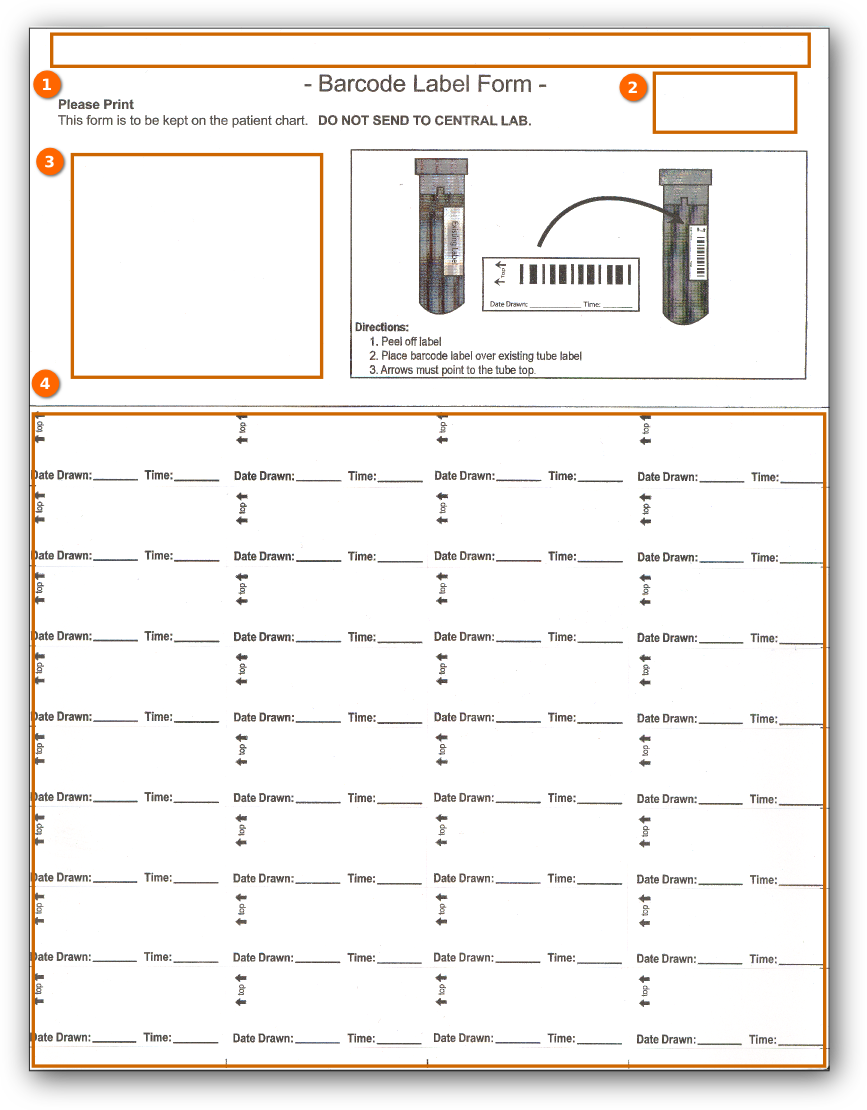
\includegraphics[width=0.5\textwidth]{screenshots/printer_labels/01_cbsr_patient_label_sheet}
  \end{center}
  \caption{CBSR Patient Label sheet.}
  \label{fig:cbsr_patient_label_sheet}
  \vspace{-15pt}
\end{wrapfigure}

Each patient label contains a 1D barcode for the patient number and a unique 2D
Data Matrix barcode for the specimen ID. Each specimen ID is unique amongst any
patient labels printed in the past and in the future. Also, the specimen ID is
unique across patients such that two patients will never have the same specimen
ID.

Figure \ref{fig:cbsr_patient_label_sheet} shows a blank CBSR Patient Label
sheet. It is a letter sized, 8$\frac{1}{2}$'' x 11'', sheet that
feeds into any printer.

The regions highlighted in orange are:
\begin{enumerate}
  \item The title area. Clinics and sites can customize their labels by
    printing their own title text.
  \item The logo region. A custom logo or graphic can be printed on the label.
  \item Patient information section. Up to 3 custom fields can be printed in
    this region.
  \item The individual patient labels that contain a 1D barcode for the patient
    number and a 2D barcode for the specimen ID. There are 32 labels in total.
\end{enumerate}

\subsection{Patient Label Information}

To print one of these sheets, some information must first be entered. Select
\texttt{Printer Labels} $\to$ \texttt{Patient Labels} from the main menu.

\begin{figure}[H]
  \centering
  \scalebox{0.35}
	   { \includegraphics*{screenshots/printer_labels/02_patient_labels_menu_item} }
	   \caption{Patient Labels menu item.}
	   \label{fig:patient_labels_menu_item}
\end{figure}

Figure \ref{fig:patient_label_form} shows the form that is displayed.

\begin{figure}[H]
  \centering
  \scalebox{0.45}
	   { \includegraphics*{screenshots/printer_labels/03_patient_label_form} }
	   \caption{Patient Label entry form.}
	   \label{fig:patient_label_form}
\end{figure}

In the \textbf{branding section}, the following information should be entered.

\begin{description}
\item[Title] This is the string that will be printed in the label sheet's title
  area. See area \textbf{1} in figure \ref{fig:cbsr_patient_label_sheet}. This field
  is optional.
\item[Logo] This allows you to select a graphic logo to be printed on the
  sheet. Press the \fbox{Browse} button to select the graphic file from your
  computer. This field is optional.
\item[Template] This is the template that specifies the position and dimension
  information for where to print information on the sheet. See section
  \ref{sec:label_templates} for more information on templates. The template
  name is a \textbf{required} field.
\item[Intended Printer] this is the printer the template was created for. You
  may have more than one template to select from. Each template is meant for a
  specific printer. This is displayed for informational purposes only.
\item[Printer] This pull down menu allows you to select the printer to use when
  printing the sheets. This menu displays the printers that have been
  configured on your computer. The printer is a \textbf{required} field.
\end{description}

In the \textbf{Patient Information} section the following information should be
entered.

\begin{description}
\item[Patient Number] Type the patient's number into this box. Any characters
  can be used up to a maximum of 14. This field cannot be left empty.
\item[Custom Fields] Three custom fields can be enabled to print on the
  label sheet. The text box on the left is the field name and the text box on
  the right is its corresponding value. In this example, the following are used
  for custom fields:

  \begin{center}
    \begin{tabular}{ | l | l | l | p{5cm} |}
      \hline
      Custom Field & Name & Value \\ \hline
      1 & Patient Name & Jonh Doe \\ \hline
      2 & PHN & 5555-5555-5555 \\ \hline
      3 & Patient Type & Control Patient \\
      \hline
    \end{tabular}
  \end{center}

  The checkboxes to the left of the field name can be used to enable / disable
  the printing of the field. The checkboxes in the middle are used to enable /
  disable printing of the value. The checkboxes on the right are used to enable
  / disable printing a 1D barcode for the corresponding field value. For
  example a 1D barcode will be printed with the text \emph{John Doe} encoded on
  it.
\end{description}

The above two sections are printed on the top portion of the label
sheet. Figure \ref{fig:printed_sheet_top} show what is printed for the values
entered into the form in figure \ref{fig:patient_label_form}.

\begin{figure}[H]
  \centering
  \scalebox{0.6}
	   { \includegraphics*{screenshots/printer_labels/04_printed_patient_labels_top} }
	   \caption{Top portion of printed patient label sheet.}
	   \label{fig:printed_sheet_top}
\end{figure}

The \textbf{Additional Configuration} section is for text to print under the
barcodes on each patient label. In the example shown in figure
\ref{fig:patient_label_form} the text \emph{Sp. Type} with underscore
characters will be printed as shown in \ref{fig:sp_type_single_label}.

\begin{figure}[H]
  \centering
  \scalebox{1.0}
	   { \includegraphics*{screenshots/printer_labels/05_single_label} }
	   \caption{Text printed on each label.}
	   \label{fig:sp_type_single_label}
\end{figure}

To print a sheet of labels you can press the \textbf{Print} button at the top
left of the form. Alternatively, instead of printing a sheet you can export the
sheet to a PDF file by pressing the \fbox{Export to PDF} button.

\subsection{Label Templates}
\label{sec:label_templates}

Select \texttt{Printer Labels} $\to$ \texttt{Label Templates} from the main
menu to see the form shown in figure \ref{fig:label_templates_form}.

\begin{figure}[H]
  \centering
  \scalebox{0.45}
	   { \includegraphics*{screenshots/printer_labels/06_label_templates_form} }
	   \caption{Label templates form.}
	   \label{fig:label_templates_form}
\end{figure}

The label template \emph{Patient with Source Specimen Label Template} is
already configured on the server for all users. This default template
tells the software where to print the information on the label sheet.  For your
printer, it is possible that the default template does not print the information
at the correct positions. You can create a new template by copying the default
template and adjusting the settings for your printer.

You may need to define templates for each printer that your computer can
access. To copy a template select the template you want to copy and press the
\fbox{Copy} button. You can also create a fresh template by pressing the
\fbox{New} button. In the future, you may want to delete an old template that
is no longer in use. This can be done by selecting the template to be deleted
and pressing the \fbox{Delete} button. To save your settings to the template
you can press the \textbf{Confirm} button at the top left of the form.

The settings for a template are:
\begin{description}
\item[Template Name] A descriptive name for the template. It is a good idea to
  include the name of the printer the template is intended for.
\item[Jasper Configuration] For patient labels you should always select the
\emph{Patient with Source Specimens Jasper Template}. This template is defined
by default on the server. For more information see section \ref{sec:jasper_templates}.
\item[Intended Printer] the name of the printer the template is intended for.
\item[Configuration] Allows for adjustments to the positions for the items to be printed.
\end{description}

Each 1D and 2D barcode item on the sheet has a \textbf{horizontal offset},
\textbf{vertical offset}, \textbf{width} and \textbf{height}. All measurements
are in millimetres. The \textbf{Patient Info} group corresponds to section
\textbf{3} in figure \ref{fig:cbsr_patient_label_sheet}. The \textbf{Barcodes}
group corresponds to the 32 patient labels. The labels are numbered starting at
the top left and ending at the bottom right. Under this group there is a
\textbf{General} node that controls the position of the patient 1D barcode, the
specimen ID 2D barcode, and the custom text position for all 32 labels. In
addition, each label can control the position of the same 3 items
individually. If values are entered here they are added to the values in the
general group. To move something to the left then use a negative value.

For example if the general barcode settings are the ones shown in the
\textbf{General} node in the tree in figure \ref{fig:label_templates_form}, and
the settings for barcode 001 are changed to those shown in figure
\ref{fig:label_templates_form}, then the patient barcode is printed 10 mm from
the left edge and 7 mm from the top edge.

Note that width and height is only applicable to 1D and 2D barcodes. For items
with the text \textbf{Text} in the name the widht and the height are ignored.

\section{Advanced Usage - Jasper Templates}
\label{sec:jasper_templates}

\emph{There is no need for the average user to change the Jasper
  Templates. The Jasper configuration templates feature should only be used by
site administrators.}

The printing of the information on a patient label sheet is managed by
JasperReports. To print the sheet there is information that must be given to
JasperReports for it to print correctly. This template holds the information and
is customized for the patient labels sheet.

In the future, additional label sheets may be printed by the Java client. Future
label sheets will have their own Jaspser templates.

%%% Local Variables:
%%% compile-command: "make -k"
%%% End:


\backmatter
\end{document}
